\documentclass[]{report}
\usepackage{lmodern}
\usepackage{amssymb,amsmath}
\usepackage{ifxetex,ifluatex}
\usepackage{fixltx2e} % provides \textsubscript
\ifnum 0\ifxetex 1\fi\ifluatex 1\fi=0 % if pdftex
  \usepackage[T1]{fontenc}
  \usepackage[utf8]{inputenc}
\else % if luatex or xelatex
  \ifxetex
    \usepackage{mathspec}
  \else
    \usepackage{fontspec}
  \fi
  \defaultfontfeatures{Ligatures=TeX,Scale=MatchLowercase}
\fi
% use upquote if available, for straight quotes in verbatim environments
\IfFileExists{upquote.sty}{\usepackage{upquote}}{}
% use microtype if available
\IfFileExists{microtype.sty}{%
\usepackage{microtype}
\UseMicrotypeSet[protrusion]{basicmath} % disable protrusion for tt fonts
}{}
\usepackage[margin=1in]{geometry}
\usepackage{hyperref}
\hypersetup{unicode=true,
            pdftitle={Informe prototipo},
            pdfauthor={SmartCrop},
            pdfborder={0 0 0},
            breaklinks=true}
\urlstyle{same}  % don't use monospace font for urls
\usepackage{natbib}
\bibliographystyle{apalike}
\usepackage{longtable,booktabs}
\usepackage{graphicx,grffile}
\makeatletter
\def\maxwidth{\ifdim\Gin@nat@width>\linewidth\linewidth\else\Gin@nat@width\fi}
\def\maxheight{\ifdim\Gin@nat@height>\textheight\textheight\else\Gin@nat@height\fi}
\makeatother
% Scale images if necessary, so that they will not overflow the page
% margins by default, and it is still possible to overwrite the defaults
% using explicit options in \includegraphics[width, height, ...]{}
\setkeys{Gin}{width=\maxwidth,height=\maxheight,keepaspectratio}
\IfFileExists{parskip.sty}{%
\usepackage{parskip}
}{% else
\setlength{\parindent}{0pt}
\setlength{\parskip}{6pt plus 2pt minus 1pt}
}
\setlength{\emergencystretch}{3em}  % prevent overfull lines
\providecommand{\tightlist}{%
  \setlength{\itemsep}{0pt}\setlength{\parskip}{0pt}}
\setcounter{secnumdepth}{5}
% Redefines (sub)paragraphs to behave more like sections
\ifx\paragraph\undefined\else
\let\oldparagraph\paragraph
\renewcommand{\paragraph}[1]{\oldparagraph{#1}\mbox{}}
\fi
\ifx\subparagraph\undefined\else
\let\oldsubparagraph\subparagraph
\renewcommand{\subparagraph}[1]{\oldsubparagraph{#1}\mbox{}}
\fi

%%% Use protect on footnotes to avoid problems with footnotes in titles
\let\rmarkdownfootnote\footnote%
\def\footnote{\protect\rmarkdownfootnote}

%%% Change title format to be more compact
\usepackage{titling}

% Create subtitle command for use in maketitle
\newcommand{\subtitle}[1]{
  \posttitle{
    \begin{center}\large#1\end{center}
    }
}

\setlength{\droptitle}{-2em}
  \title{Informe prototipo}
  \pretitle{\vspace{\droptitle}\centering\huge}
  \posttitle{\par}
  \author{SmartCrop}
  \preauthor{\centering\large\emph}
  \postauthor{\par}
  \predate{\centering\large\emph}
  \postdate{\par}
  \date{2017-05-15}

\usepackage{booktabs}
\usepackage{amsthm}
\makeatletter
\def\thm@space@setup{%
  \thm@preskip=8pt plus 2pt minus 4pt
  \thm@postskip=\thm@preskip
}
\makeatother

\begin{document}
\maketitle

{
\setcounter{tocdepth}{1}
\tableofcontents
}
\chapter{Resumen}\label{resumen}

Este documento corresponde a un informe prototipo para presentar como
información complementaria para postulación a Proyecto PRAE-BíoBío. El
informe presenta los resultados obtenidos a nivel de desarrollo de
pre-servicio mínimo viable del análisis de las condiciones
vegetacionales en un predio en base a información satelital como soporte
a la toma de decisiones para los agricultores. En este caso se considera
una fecha puntual, correspondiente al \textbf{20 de diciembre 2016}. En
este prototipo se considera un predio en el cual se cultiva Maiz ubicado
en la comuna de San Carlos. El informe esta estructurado con las
secciones:

\begin{enumerate}
\def\labelenumi{\arabic{enumi}.}
\tightlist
\item
  \protect\hyperlink{DescripcionVIs}{Descripción índices vegetacionales}
\item
  \protect\hyperlink{SelecPredios}{Selección de predios}
\item
  \protect\hyperlink{indicesVeg}{Índices vegetacionales}
\item
  \protect\hyperlink{AnalisisDatos}{Análisis de datos}
\end{enumerate}

\hypertarget{DescripcionVIs}{\chapter{Descripción Índices
Vegetacionales}\label{DescripcionVIs}}

En esta sección se describen las principales caracteristicas de los
índices usados para el monitoreo del estado vegetacional de lso
cultivos.

\begin{enumerate}
\def\labelenumi{\arabic{enumi}.}
\item
  \textbf{Índice de vegetación de diferencia normalizada (NDVI):} Es un
  índice usado para estimar la cantidad, calidad y desarrollo de la
  vegetación con base a la medición, por medio de sensores remotos .
\item
  \textbf{Índice diferencial de agua normalizado (NDWI):} Se utiliza
  como una medida de la cantidad de agua que posee la vegetación o el
  nivel de saturación de humedad que posee el suelo.
\item
  \textbf{Borde Rojo - Índice Normalizado de Diferencia de Vegetación
  (RE-NDVI):} Se utiliza como una medida de si la vegetación se
  encuentra saludable. Es similar al NDVI, pero utiliza las bandas de
  infrarojo cercano y de borde rojo.
\end{enumerate}

\hypertarget{SelecPredios}{\chapter{Selección de
Predios}\label{SelecPredios}}

En esta sección se muestra la forma en la cual el cliente podrá
seleccionar su área de interes materia del servicio solicitado.

\begin{figure}

{\centering \includegraphics[width=1\linewidth]{bookdown-demo_files/figure-latex/selection-1} 

}

\caption{Índices vegetacionales}\label{fig:selection}
\end{figure}

\hypertarget{indicesVeg}{\chapter{Índices
vegetacionales}\label{indicesVeg}}

\begin{figure}

{\centering 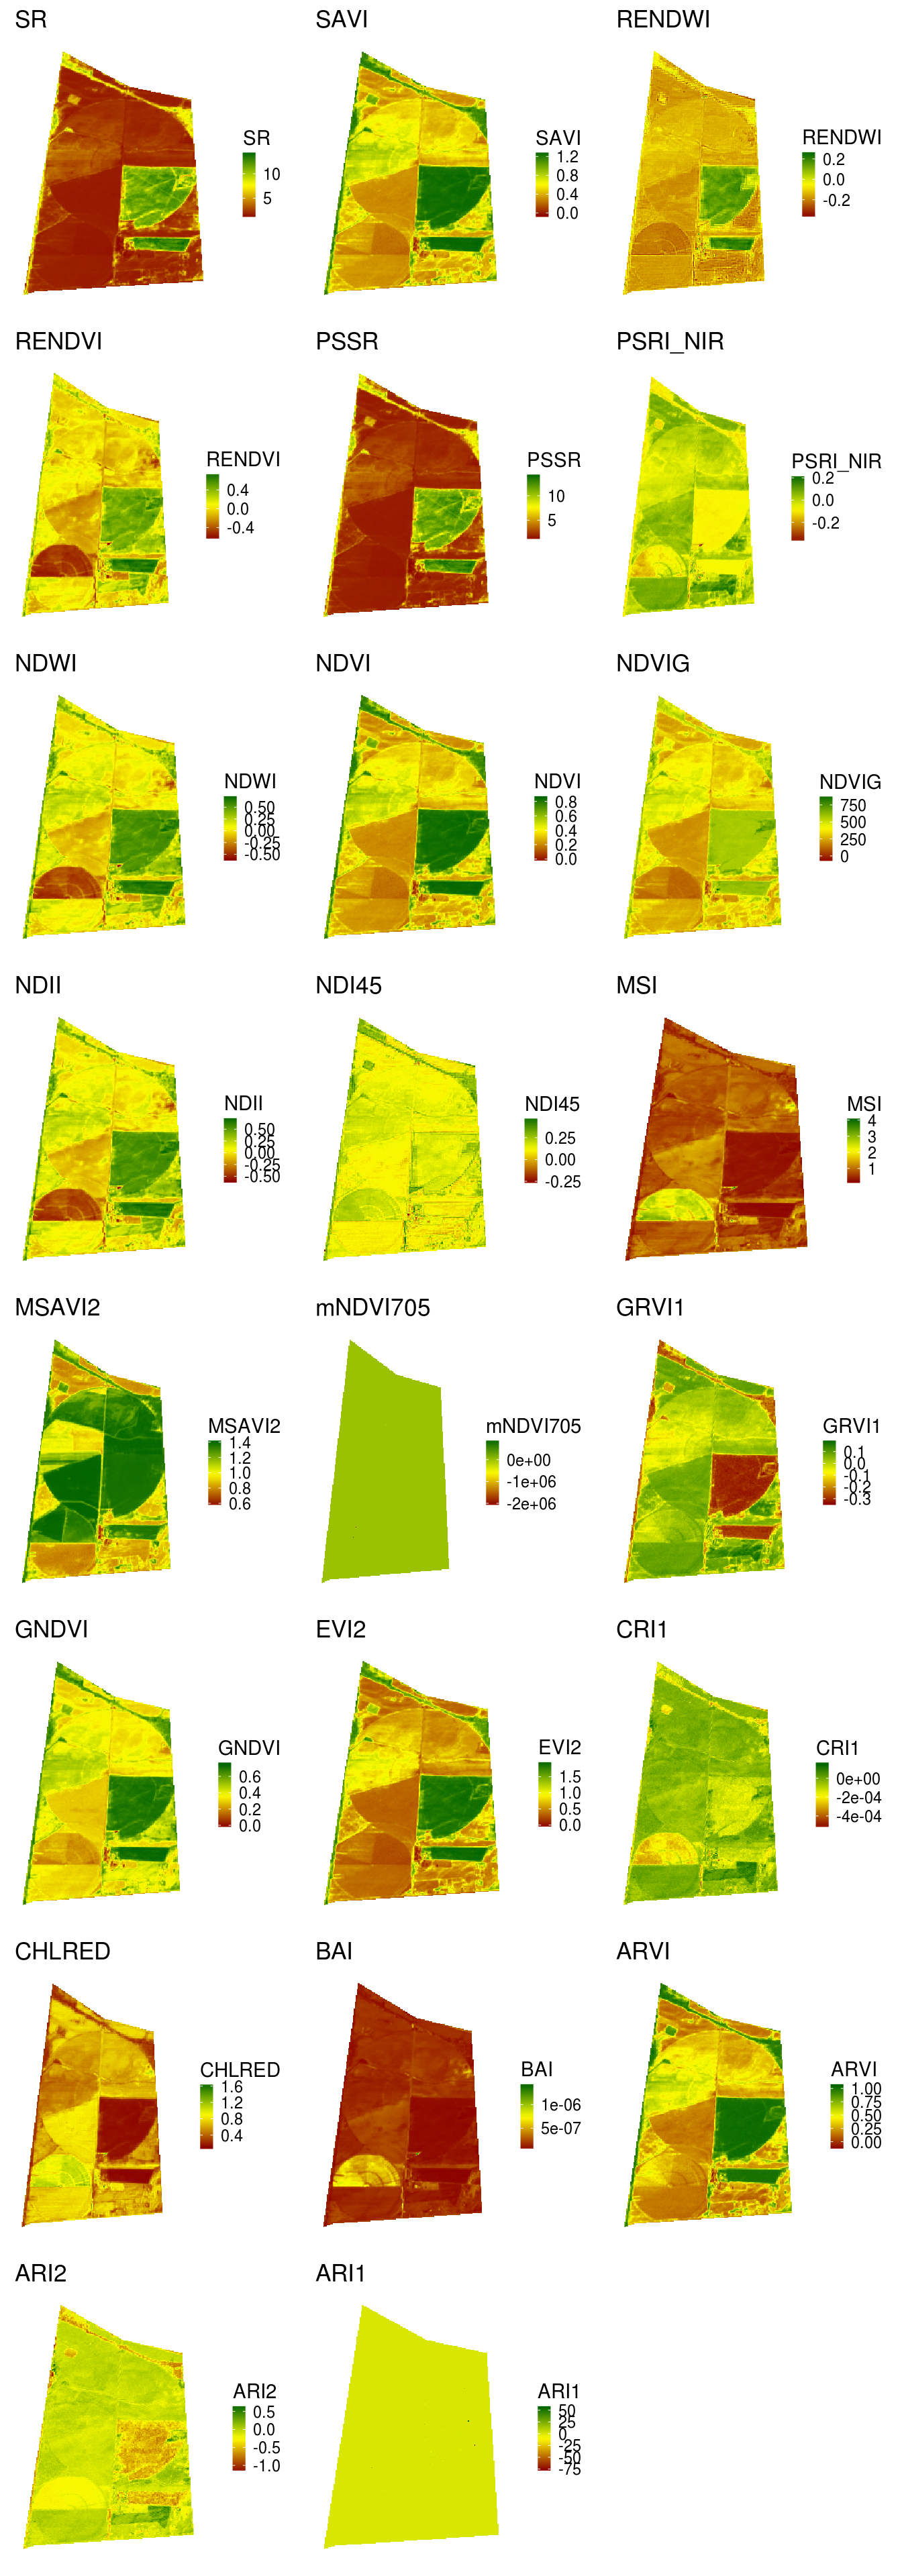
\includegraphics[width=1\linewidth]{bookdown-demo_files/figure-latex/Fron-1} 

}

\caption{Índices vegetacionales}\label{fig:Fron}
\end{figure}

\bibliography{packages.bib,book.bib}


\end{document}
